\documentclass[cplx.tex]{subfiles}

\begin{document}
\part{Integral Transforms}
\chapter{}
\begin{align}
    g(w) &= \int_a^b K(w,x)f(x)\,dx
\end{align}
\begin{itemize}
    \item $f(x),g(w)$: complex functions of a real variable
    \item $K(w,x)$ : kernal propagator
    \item $a,b$ can be (and every often are) $\pm \infty$
    \item $g(w) = Tf(w)$
    \item $F \to^T F$ 
    \item $f \to q = Tf$
\end{itemize}
The transformation is linear and invertible:
\begin{align}
    T[a_1f_1 + a_2f_2] &= a_1T[f_1] + a_2T[f_2] \\
    f(x) &= T^{-1}g(w) 
\end{align}
\begin{equation*}
    \begin{matrix} \text{Original problem (complicated)} & \to & \text{Solution} \\ T\downarrow & & \uparrow T^{-1} \\ \text{Transformed problem} & \to_{\text{easier}} & \text{Transformed solution} \end{matrix}
\end{equation*}
Two main parts of the course:
\begin{itemize}
    \item Fourier transforms
    \item Laplace transforms
\end{itemize}

\section{Fourier Transforms}
\begin{align}
    \F[f(x)](w) \equiv \tilde{f}(w) &= \frac{1}{\sqrt{2\pi}} \ifnt f(x)e^{iwx}dx
\end{align}
Requirements:
\begin{itemize}
    \item $f(x)$ is square-integrable, i.e.
        \begin{equation}
            \ifnt |f(x)|^2\,dx < \infty
        \end{equation}
    \item $f(x)$ is continuous (the transformation is invertible), i.e.
        \begin{equation}
            \F^{-1}[\tilde{f}(w)](x) = f(x) = \frac{1}{\sqrt{2\pi}} \ifnt \tilde{f}(w)e^{-iwx}dw
        \end{equation}
    \item $\frac{1}{\sqrt{2\pi}}$ is used as a normalisation factor for $\F$ and $\F^{-1}$, but different normalisation factors may be used. 
\end{itemize}
Generalisation to 3D:
\begin{equation}
    \F[f(\vr)] \equiv \tilde{f}(\vec{k}) = \frac{1}{(2\pi)^{3/2}} \int f(\vr)e^{i\vec{k}\cdot\vr} d\vr
\end{equation}

\section{Fourier Transform as a limit of Fourier series}
Consider $f(x)$ periodic in $x \in [-L,L]$.
\begin{align}
    f(x) &= a_0 + \sum_{n=1}^\infty \left[a_n\cos\left(\frac{n\pi x}{L}\right) + b_n\sin\left(\frac{n\pi x}{L}\right)\right] \\
    a_0 &= \frac{1}{2L} \int_{-L}^L f(t)\,dt \\
    a_n &= \frac{1}{L} \int_{-L}^L f(t)\cos\left(\frac{n\pi t}{L}\right)\,dt \\
    b_n &= \frac{1}{L} \int_{-L}^L f(t)\sin\left(\frac{n\pi t}{L}\right)\,dt \\
    f(x) &= \frac{1}{2L} \int_{-L}^L f(t)\,dt + \frac{1}{L} \sum_{n=1}^\infty \int_{-L}^L f(t)\left[\cos\left(\frac{n\pi t}{L}\right)\cos\left(\frac{n\pi x}{L}\right) + \sin\left(\frac{n\pi t}{L}\right)\sin\left(\frac{n\pi x}{L}\right)\right]\,dt \\
         &= \frac{1}{2L} \int_{-L}^L f(t)\,dt + \frac{1}{L}\sum_{n=1}^\infty \int_{-L}^L f(t)\cos\left(\frac{n\pi(t-x)}{L}\right)\,dt \\
         &= \frac{1}{2L} \int_{-L}^L f(t)\,dt + \frac{1}{2L}\sum_{n=1}^\infty \int_{-L}^L f(t)\left[e^{in\pi(t-x)/L} + e^{-in\pi(t-x)/L}\right] \\
    w_n &= \frac{n\pi}{L} \implies \Delta w = w_{n+1} - w_n = \frac{\pi}{L} \\
    L &\to \infty,~ \Delta w \to dw \\
    f(x) &= \sum_{n=-\infty}^\infty \frac{1}{2L} \int_{-L}^L f(t)e^{in\pi(t-x)}{L}dt \\
    \lim_{L\to\infty} f(x) &= \frac{1}{2\pi} \ifnt dw \ifnt dt f(t)e^{iw(t-x)} \\
    \frac{1}{L} &= \frac{\Delta w}{\pi} \to \frac{dw}{\pi} \\
    f(x) &= \frac{1}{\sqrt{2\pi}} \ifnt \left(\frac{1}{\sqrt{2\pi}} \ifnt f(t)e^{-iwt}dt\right)\,e^{-iwx}dw \\
         &\implies \F^{-1}[\F[f(t)](w)]
\end{align}

\section{Fourier transform of a Gaussian}
\begin{align}
    f(x) &= e^{-x^2/2} \\
    \F[f(x)](w) &= \frac{1}{\sqrt{2\pi}} \ifnt e^{-x^2/2}e^{iwx}dx \\
                &= \frac{1}{\sqrt{2\pi}} \ifnt e^{-(x-iw)^2/2}e^{-w^2/2}dx \\
                &= \frac{e^{-w^2/2}}{\sqrt{2\pi}} \ifnt e^{-(x-iw)^2/2}dx \\
                &\oint e^{-z^2/2}\,dx,~ z=x+iy
\end{align}
\begin{center}
    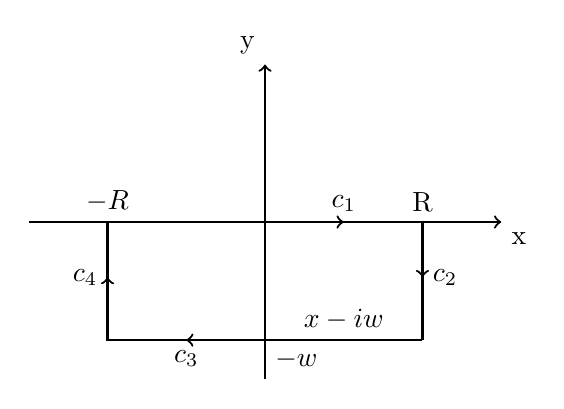
\begin{tikzpicture}
        \draw[thick,->] (-3,0) -- (3,0) node[anchor=north west] {x};
        \draw[thick,->] (0,-2) -- (0,2) node[anchor=south east] {y};
        \draw[thick,->] (0,0) -- (1,0) node[anchor=south] {$c_1$};
        \draw[thick,->] (2,0) -- (2,-0.7) node[anchor=west] {$c_2$};
        \draw[thick] (2,0) node[anchor=south] {R} -- (2,-1.5);
        \draw[thick] (2,-1.5) -- (0,-1.5) node[anchor=north west] {$-w$} node[anchor=south,midway] {$x-iw$} -- (-2,-1.5) -- (-2,0) node[anchor=south] {$-R$};
        \draw[thick,->] (0,-1.5) -- (-1,-1.5) node[anchor=north] {$c_3$};
        \draw[thick,->] (-2,-1.5) -- (-2,-0.7) node[anchor=east] {$c_4$};
    \end{tikzpicture}
\end{center}
\begin{align}
    C &= c_1 + c_2 + c_3 + c_4,~ \lim R \to \infty \\
    \oint &= \int_{c_1} + \int_{c_2} + \int_{c_3} + \int_{c_4} \\
    \int_{c_1} e^{-z^2/2}dz &= \int_{-R}^R e^{-x^2/2}dx = \sqrt{2\pi} \\
    \lim_{R\to\infty} \left(\int_{c_2}\right) &= \int_0^{-w} e^{-(x+iy)^2/2}dy = 0,~ \int_{c_4} = 0\\
    \int_{c_3} &= \int_R^{-R} e^{-(x-iw)^2/2}dx \\
    \int_{c_1} &= -\int_{c_3} \\
    \F[f(x)](w) &= e^{-w^2/2} \\
    \F[e^{-x^2/2}] &= e^{-w^2/2}
\end{align}

\chapter{}
\section{Fourier Transforms}
\begin{align}
    \F[f(x)](w) &= \frac{1}{\sqrt{2\pi}} \ifnt e^{iwx}f(x)dx \\
    \F^{-1}[\hat{f}(w)](x) &= \frac{1}{\sqrt{2\pi}} \ifnt e^{-iwx}\hat{f}(w)dw
\end{align}
1-dimensional string (wave equation):
\begin{align}
    \frac{\p^2Y(x,t)}{\p x^2} &= \frac{1}{v^2}\frac{\p^2Y(x,t)}{\p t^2} \\
    y''(x) - 4y(x) &= e^{-x^2/8}
\end{align}

\subsection{Fourier transform of a derivative}
\begin{align}
    \F\left[\frac{df(x)}{dx}\right](x) &= \frac{1}{\sqrt{2\pi}} \ifnt \frac{df(x)}{dx} e^{iwx}\,dx \\
                                       &= \frac{1}{\sqrt{2\pi}} f(x)e^{iwx}\bigg|_{-\infty}^{\infty} - \frac{1}{\sqrt{2\pi}} \ifnt f(x)iwe^{iwx}dx 
\end{align}
This implies that $f(x)$ vanishes at $-\infty$ and $\infty$.
\begin{align}
    \F\left[\frac{df(x)}{dx}\right](w) &= -iw\frac{1}{\sqrt{2\pi}} \ifnt f(x)e^{iwx}dx \\ 
    \F\left[\frac{df(x)}{dx}\right] &= -iw\F[f(x)]
\end{align}
Can generalise to the n-th derivative:
\begin{align}
    \F\left[\frac{d^nf(x)}{dx^n}\right](w) &= (-iw)^n\F[f(x)](w)
\end{align}
Differential equation in $x \to$ polynomial equation in $w$.

What about Fourier trnasform of $x^nf(x)$?
\begin{align}
    \F[xf(x)](w) &= \frac{1}{\sqrt{2\pi}} \ifnt \overbrace{e^{iwx}x}^{\frac{1}{i}\frac{de^{iwx}}{dx}}f(x)\,dx \\
                 &= \frac{1}{\sqrt{2\pi}} \frac{1}{i} \ifnt \frac{de^{iwx}}{dx}f(x)\,dx \\
                 &= \frac{-i}{\sqrt{2\pi}} \frac{d}{dw} \ifnt e^{iwx}f(x)\,dx \\
                 &= -i\frac{d}{dw} \left[\F[f(x)](w)\right]
\end{align}
And generally, 
\begin{align}
    \F[x^nf(x)](w) &= (-i)^n\frac{d^n}{dw^n} \left[\F[f(x)](w)\right]
\end{align}

\subsection{Fourier transforms and scaling}
\begin{align}
    \F[f(ax)](w) &= \frac{1}{\sqrt{2\pi}} \ifnt e^{iwx}f(ax)\,dx,~ x' = ax \\
                 &= \frac{1}{\sqrt{2\pi}} \ifnt e^{iwx'/a}f(x')\,\frac{dx'}{a} \\
                 &= \frac{1}{a}\F[f(x)]\left(\frac{w}{a}\right)
\end{align}

\subsection{Fourier transform of a translated function}
\begin{align}
    \F[f(a+x)](w) &= \frac{1}{\sqrt{2\pi}} \ifnt e^{iwx}f(a+x)\,dx,~ x' = a+x \\
                  &= \frac{1}{\sqrt{2\pi}} \ifnt e^{iw(x'-a)}f(x')\,dx \\
                  &= e^{-iwa}\F[f(x)](w) \\
    \F[e^{iax}f(x)] &= \F[f(x)](w+a)
\end{align}

\subsection{1D String Wave Equation}
\begin{align}
    \frac{\p^2Y(x,t)}{\p x^2} &= \frac{1}{v^2}\frac{\p^2 Y(x,t)}{\p t^2} \\
    \F\left[\frac{\p^2Y(x,t)}{\p x^2}\right] &= \frac{1}{v^2}\F\left[\frac{\p^2Y(x,t)}{\p t^2}\right],~ \F[Y(x,t)] \equiv \hat{Y}(w,t) \\
    (-iw)^2\hat{Y} &= \frac{1}{v^2}\frac{\p^2}{\p t^2}\hat{Y} \\
    \frac{\p^2}{\p t^2} \hat{Y} &= -(w^2v^2)\hat{Y}  \\
    \hat{Y}(w,t) &= A(w)e^{iwvt} + B(w)e^{-iwvt} \\
    Y(x,t) &= \F^{-1}[\hat{Y}](x,t) \\
           &= \frac{1}{\sqrt{2\pi}} \ifnt \left(A(w)e^{-iwx}e^{iwvt} + B(w)e^{-iwx}e^{-iwvt}\right)\,dw \\
           &= \frac{1}{\sqrt{2\pi}} \ifnt \left(A(w)e^{-iw(x-vt)} + B(w)e^{-iw(x+vt)}\right)\,dw
\end{align}

Now consider
\begin{align}
    y'' -4y &= e^{-x^2/8} \\
    \F[y''-4y] &= \F\left[e^{-x^2/8}\right],~ \F[y] \equiv \hat{y} \\
    (-iw)^2\hat{y} - 4\hat{y} &= \F\left[e^{-x'2/2}\right],~ x' \equiv \frac{x}{2} \\
                              &= 2e^{-2w^2} \\
    \hat{y} &= \frac{-2e^{-2w^2}}{4+w^2} \\
    y &= \F^{-1}[\hat{y}] \\
    y(x) &= \frac{1}{\sqrt{2\pi}} \ifnt \left(\frac{-2e^{-2w^2}}{4+w^2}\right)e^{-iwx}dw 
\end{align}
Solution to the homogeneous equation: $y = y_h + y_p$ (above is particular).
\begin{align}
    y'' &- 4y = 0 \\
    y &= A(x)e^{2x} + B(x)e^{-2x}
\end{align}

What about:
\begin{align}
    y'' - 4y &= \cos(x) \\
    \F[\cos(x)] &= \frac{1}{\sqrt{2\pi}} \ifnt e^{iwx}\cos(x)\,dx
\end{align}
We have an issue here as $\cos(x)$ is not square integrable.

\chapter{}
Dirac $\delta$ function such that
\begin{align}
    \delta(x) &= 0, x \neq 0\\
    \ifnt \delta(x)\,dx &= 1 \\
    \ifnt \delta(x)f(x)\,dx &= f(0)
\end{align}
Think of 
\begin{align}
    f_n(x) &\equiv \frac{n}{\sqrt{\pi}} e^{-n^2x^2}
\end{align}
Satisfies the properties of $f(x)$ where $\lim_{n\to\infty}$
\begin{align}
    \lim_{n\to\infty} \left(\ifnt \frac{n}{\sqrt{\pi}} e^{-n^2x^2}\,dx\right) &= \lim_{n\to\infty} \frac{n}{\sqrt{\pi}} \frac{\sqrt{\pi}}{n} = 1
\end{align}
Imagine graphically as Gaussians centered on $x=0$ that slowly gets sharper and sharper towards delta spike.
\begin{align}
    g_n(x) &= \frac{n}{\pi}\frac{1}{1+n^2x^2}
\end{align}
Properties:
\begin{align}
    \delta(x) &= \delta(-x) \\
    \ifnt \delta(x-a)f(x) &= \ifnt \delta(x-a)f(a) \\
                          &= f(a) \ifnt \delta(x-a)\,dx = f(a) \\
    \delta[g(x)] &= \sum_{x_i, \text{ zeros of g}} \frac{\delta(x-x_i)}{|g'(x_i)|}
\end{align}
$g(x)$ has at most simple zeros.
\begin{align}
    \ifnt \delta[g(x)]\,dx &= \ifnt \delta[(x-x_i)g'(x_i)]\, dx \\
    x' &= (x-x_i)g'(x_i) \\
    dx &= \frac{dx'}{|g'(x_i)|} \\
    \delta(ax) &= \frac{\delta(x)}{a}
\end{align}
$\delta$ is differentiable
\begin{align}
    \ifnt \delta'(x)f(x)\,dx &= \cancel{f(x)\delta(x)\big|_{-\infty}^{\infty}} - \ifnt \delta(x)f'(x)\,dx \\
                             &= (-1)f'(0)
\end{align}
Generalising to $n$-th order:
\begin{align}
    \ifnt \delta^{(n)}(x)f(x)\,dx &= (-1)^nf^{(n)}(0)
\end{align}

The Heaviside step function is the primitive of $\delta(x)$
\begin{align}
    \Theta(x) &= \begin{cases} 1 & x \geq 0 \\ 0 & x < 0 \end{cases} \\
    \ifnt \Theta'(x)f(x)\,dx &= \ifnt \delta(x)f(x)\,dx
\end{align}

\section{Fourier Representation of delta function}
\begin{align}
    \F[\delta(x)] \equiv \hat{\delta}(w) &= \frac{1}{\sqrt{2\pi}} \ifnt \delta(x) e^{iwx}\,dx \\
                         \hat{\delta}(w) &= \frac{1}{\sqrt{2\pi}} \\
    \F^{-1}[\hat{\delta}(w)] = \delta(x) &= \frac{1}{\sqrt{2\pi}} \ifnt \frac{1}{\sqrt{2\pi}}e^{-iwx}\,dw \\
    \delta(x) &= \frac{1}{2\pi} \ifnt e^{-iwx}\,dw \\
    \delta(x) &= \delta(-x) \\
    \delta(x) &= \frac{1}{2\pi} \ifnt 1\cdot e^{iwx}\,dw = \frac{1}{\sqrt{2\pi}}\F[1] \\
    \F[1] &= \sqrt{2\pi}\delta(x)
\end{align}
Also:
\begin{align}
    \F[e^{iax}] &= \frac{1}{\sqrt{2\pi}} \ifnt e^{iax}e^{iwx}\,dx,~ |e^{iax}| = 1 \\
                &= \sqrt{2\pi}\delta(w+a)
\end{align}

\section{Convolutions}
\begin{align}
    f(x) &\to \hat{f}(w) \\
    g(x) &\to \hat{g}(w) \\
    f(x)*g(x) &\equiv \frac{1}{\sqrt{2\pi}} \ifnt g(y)f(x-y)\,dy \\
\end{align}
This is the Convolution.
\begin{align}
    \frac{1}{\sqrt{2\pi}} \ifnt g(y)f(x-y)\,dy &= \frac{1}{\sqrt{2\pi}} \ifnt g(y)\left(\frac{1}{\sqrt{2\pi}} \ifnt \hat{f}(w)e^{-iw(x-y)}dw\right)\,dy \\
                                               &= \frac{1}{\sqrt{2\pi}} \ifnt \hat{f}(w)\left(\underbrace{\frac{1}{\sqrt{2\pi}} \ifnt g(x)e^{iwy} dy}_{\hat{g}(w)}\right)\,e^{-iwx} dw \\
                                               &= \frac{1}{\sqrt{2\pi}} \ifnt \hat{f}(w)\hat{g}(w)e^{-iwx}\,dw \\
    f(x)*g(x)  &= \F^{-1}[\hat{f}(w)\hat{g}(w)] \\
    \F[f(x)*g(x)] &= \hat{f}(w)\hat{g}(w)
\end{align}

\begin{example}
\begin{align}
    f''(x) &- f(x) = e^{-x^2} \\
    f(x) &= f_h(x) + f_p(x) 
\end{align}
Solution to the Homogeneous equation:
\begin{align}
    f''(x) &- f(x) = 0 \\
    f_h(x) &= Ae^{-x} + Be^x \\
\end{align}
Now for the particular:
\begin{align}
    \F[f''(x) - f(x)] &= \F[e^{-x^2}] \\
    (-iw)^2\hat{f}(w) - \hat{f}(w) &= \F[e^{-x^2}] \\
    \hat{f}(w) &= \F[e^{-x^2}] \frac{-1}{1+w^2} \\
               &= -\F[e^{-x^2}] \F[\textit{something}] \\
               &= -\F[e^{-x^2}*\textit{something}] \\
    f(x) &= -e^{-x^2}*\textit{something} \\
    \textit{something} &= \F^{-1}\left[\frac{1}{1+w^2}\right] \\
    \F^{-1}\left[\frac{1}{1+w^2}\right] &= \frac{1}{\sqrt{2\pi}} \ifnt \frac{1}{1+w^2}e^{-iwx}\,dw
\end{align}
Poles at $w = \pm i$.
$x>0$, $|e^{-iwx}| = |e^{-iw_\R x}e^{w_I x}| = e^{w_I x}$.
If $x >0$, integrating on lower half of the plane, so can apply residue theorem for $w = -i$.
\begin{align}
    \F^{-1}\left[\frac{1}{1+w^2}\right] &= \frac{1}{\sqrt{2\pi}} 2\pi i\left(-\text{Res}\left(\frac{e^{-iwx}}{1+w^2}\right)_{w=-i}\Bigg|_{x\geq 0} + \text{Res}\left(\frac{e^{-iwx}}{1+w^2}\right)_{w=i}\Bigg|_{x<0}\right) \\
                                        &= \sqrt{\frac{\pi}{2}}\left(e^{-x}\Big|_{x\geq 0} + e^x\Big|_{x<0}\right) = \sqrt{\frac{\pi}{2}}e^{-|x|} \\
    \F^{-1}\left[\frac{1}{1+w^2}\right] &= \sqrt{\frac{\pi}{2}} e^{-|x|} \\
    f(x) &= -e^{-x^2}*\sqrt{\frac{\pi}{2}}e^{-|x|} \\
         &= -\frac{1}{\sqrt{2\pi}} \ifnt e^{-y^2}\sqrt{\frac{\pi}{2}} e^{-|x-y|}dy
\end{align}
\end{example}

\chapter{}
\begin{align}
    \F[f(x)](w) &= \frac{1}{\sqrt{2\pi}} \ifnt f(x)e^{iwx}dx
\end{align}

\section{Parseval's Theorem}
\begin{align}
    \ifnt f(x)^*g(x)\,dx &= \ifnt \hat{f}(w)^*\hat{g}(w)\,dw \\
    \ifnt |f(x)|^2\,dx &= \ifnt |\hat{f}(w)|^2\,dw,~ f(x) = g(x)
\end{align}
This is useful in Quantum Mechanics to show the wavefunction of a particle makes sense in momentum-space as well.
\begin{align}
    \ifnt f(x)^*g(x)\,dx &= \ifnt \left(\F^{-1}[\hat{f}(w)]\right)^*\F^{-1}[\hat{g}(w)]\,dx \\
                         &= \ifnt \left(\frac{1}{\sqrt{2\pi}} \ifnt \hat{f}(w)e^{-iwx}\,dw\right)^* \left(\frac{1}{\sqrt{2\pi}} \ifnt \hat{g}(w')e^{-iw'x}\,dw'\right)\,dx \\
                         &= \frac{1}{2\pi} \int dw \int dw' \ifnt dx\; \hat{f}(w)^*\hat{g}(w')e^{-ix(w'-w)} \\
                         &= \int dw \int dw' \hat{f}(w)^*\hat{g}(w')\delta(w'-w) \\
                         &= \ifnt \hat{f}(w)^* \hat{g}(w)\,dw
\end{align}

\begin{example}
\begin{align}
    I &= \ofnt \frac{dw}{(a^2+w^2)^2} \\
    \F^{-1}\left[\frac{1}{1+k^2}\right] &= \sqrt{\frac{\pi}{2}} e^{-|x|} \\
    I &= \frac{1}{2a^3} \ifnt \frac{dk}{(1+k^2)^2},~ k = \frac{w}{a} \\
      &= \frac{1}{2a^3} \ifnt \left(\sqrt{\frac{\pi}{2}} e^{-|x|}\right)^*\left(\sqrt{\frac{\pi}{2}} e^{-|x|}\right) dx \\
      &= \frac{1}{2a^3}\frac{\pi}{2} \ifnt \left(e^{-|x|}\right)^2\,dx \\
      &= \frac{1}{2a^3}\frac{\pi}{2} \times 2 \ofnt e^{-|x|}\,dx = \frac{\pi}{4a^3}
\end{align}
\end{example}

\section{Fourier transform and integral equations}
\begin{align}
    f(x)*g(x) &= \frac{1}{\sqrt{2\pi}} \ifnt g(y)f(x-y)\,dy
\end{align}

\begin{example}
\begin{align}
    h(x) &= e^{i3x} + \ifnt e^{-|y|}h(x-y)\,dy \\
    \hat{h}(w) &= \sqrt{2\pi}\delta(w+3) + \sqrt{2\pi}\F[e^{-|x|}]\hat{h}(w) \\
               &= \sqrt{2\pi}\delta(w+3) + \frac{2}{1+w^2}\hat{h}(w) \\
               &= \sqrt{2\pi}\delta(w+3) \left(1 - \frac{2}{1+w^2}\right)^{-1} \\
    h(x) &= \frac{1}{\sqrt{2\pi}} \ifnt \sqrt{2\pi} \delta(w+3) \left(1 - \frac{2}{1+w^2}\right)^{-1} e^{-iwx}\, dw \\
         &= \frac{5}{4}e^{i3x}
\end{align}
\end{example}

\section{Discrete Fourier Transform}
\begin{equation}
    h(t) \to \hat{h}(w)
\end{equation}
Frequency decomposition, period $h(t)$, $T$.
Meausre $h(t)$ at $t_i = t_0\cdots t_{2N}$.
Discrete fourier transform:
\begin{align}
    \hat{h}(w_p) &= \frac{1}{\sqrt{2N}} \sum_{j=0}^{2N-1} h_je^{iw_pt_j} \\
    t_j &= \frac{T}{2N}j,~ w_p = \frac{2\pi}{T}p
\end{align}
This can be inverted to construct a continuous function of $t$:
\begin{align}
    h^{DFT}(t) &= \frac{1}{\sqrt{2N}} \sum_{p=0}^{2N-1} \hat{h}(w_p)e^{-iw_pt} \\
    h^{DFT}(t) &\neq h(t)
\end{align}
They have the same periodic properties, $h^{DFT}$ converges to $h(t)$ in the limit where $j\to\infty$.

\subsection{Fourier Matrix}
\begin{align}
    \begin{pmatrix} \hat{h}_0 \\ \vdots \\ \hat{h}_{2N-1} \end{pmatrix} &= \left(\frac{e^{iw_pt_j}}{\sqrt{2N}}\right)_{pj}\begin{pmatrix} h_0 \\ \vdots \\ h_{2N-1}\end{pmatrix} \\
    \left(\frac{e^{iw_pt_j}}{\sqrt{2N}}\right) &= \left(\frac{e^{i\pi/N pj}}{\sqrt{2N}}\right)
\end{align}

\begin{example}
\begin{align}
    h(t) &= \cos(t),~ T = 2\pi \\
    h(0) &= 1,~ t_0 = 0 \\
    h(t_1) &= 0,~ t_1 = \frac{\pi}{2} \\
    h(t_2) &= -1,~ t_2 = \pi \\
    h(t_3) &= 0,~ t_3 = \frac{3\pi}{2} \\
    w_p &= \frac{2\pi}{T}p = p \\
    w_0 &= 0,~  w_1 = 1, \cdots,~ N = 2 \\
    \begin{pmatrix} \hat{h}_0 \\ \hat{h}_1 \\ \hat{h}_2 \\ \hat{h}_3 \end{pmatrix} &= \frac{1}{2}\begin{pmatrix} 1 & 1 & 1 & 1 \\ 1 & i & -1 & -i \\ 1 & -1 & 1 & -1 \\ 1 & -i & -1 & i \end{pmatrix}\begin{pmatrix} 1 \\ 0 \\ -1 \\ 0\end{pmatrix} = \begin{pmatrix} 0 \\ 1 \\ 0 \\ 1 \end{pmatrix} \\
    h(t) &= \frac12 \sum_{p=0}^3 \hat{h}_p e^{-w_p t} = \frac12\left(e^{-it} + e^{-3it}\right) \\
    h^{DFT}(t) &= \frac12 \left(\cos(t) + \cos(3t)\right) \neq h(t) = \cos(t)
\end{align}
\end{example}

\chapter{}
\section{Laplace Transforms}
\begin{align}
    \La[f(t)](s) = \bar{f}(s) &= \ofnt f(t)e^{-ts}\,dt
\end{align}
Convergence $\implies \bar{f}(s)$ not necessarily defined in the whole range of $s$.
Typically, since $t>0 \implies s>0$.

\begin{example}
    \begin{align}
        \La[1] &= \ofnt e^{-ts}dt = -\frac{1}{s}e^{-ts}\big|_0^\infty \\
               &= \frac{1}{s},~ s>0
    \end{align}
\end{example}

\begin{example}
    \begin{align}
        f(t) &= e^{at}, a>0 \\
        \La[e^{at}] &= \ofnt e^{at}e^{-st}dt \\
                    &= -\frac{1}{s-a} e^{-(s-a)t}\big|_0^\infty \\
                    &= \frac{1}{s-a},~ s>a
    \end{align}
\end{example}

\section{Relation between Laplace and Fourier transforms}
\begin{align}
    \La[f(t)] &= \ofnt f(t)e^{-st}dt,~ s=x+iy \\
              &= \ofnt f(t)e^{-(x+iy)t}dt \\
              &= \ofnt f(t)e^{-xt}e^{-iyt}dt \\
              &= \frac{1}{\sqrt{2\pi}} \ifnt \sqrt{2\pi}f(t)e^{-xt}\Theta(t)e^{-iyt}dt \\
              &= \F^{-1}\left[\sqrt{2\pi}f(t)e^{-xt}\Theta(t)\right]
\end{align}

Consider
\begin{align}
    f(t) &= \cosh(kt) = \frac{e^{kt} + e^{-kt}}{2} \\
    \La[f(t)] &= \frac12\Bigg(\underbrace{\frac{1}{s-k}}_{s>k} + \underbrace{\frac{1}{s+k}}_{s+k>0}\Bigg) = \underbrace{\frac{s}{s^2-k^2}}_{s>|k|}
\end{align}

\section{Laplace Transform and Derivatives}
\begin{align}
    \La\left[\frac{df}{dt}\right] &= \ofnt \frac{df}{dt}e^{-st}dt \\
                                  &= f(t)e^{-st}\big|_0^\infty + s\ofnt f(t)e^{-st}dt \\
                                  &= -f(0) + s\La[f(t)](s) \\
    \La\left[\frac{d^2f}{dt^2}\right] &= \La\left[\frac{d}{dt}\left(\frac{df}{dt}\right)\right] \\
                                      &= -f'(0) + s\La\left[\frac{df}{dt}\right] \\
                                      &= -f'(0) - sf(0) + s^2\La[f(t)](s) \\
    \La\left[\frac{d^nf}{dt^n}\right] &= s^n\La[f(t)](s) - \sum_{k=0}^{n-1} s^{n-1-k}f^{(k)}(0)
\end{align}

Now consider:
\begin{align}
    \La[\sinh(kt)] &= \frac{1}{k}\La\left[\frac{d}{dt}\cosh(kt)\right] \\
                   &= \frac{1}{k}\left(s\La[\cosh(kt)] - \cosh(0)\right) \\
                   &= \frac{1}{k} \Bigg(s\underbrace{\frac{s}{s^2-k^2}}_{s>|k|} - 1\Bigg) = \underbrace{\frac{k}{s^2-k^2}}_{s>|k|}
\end{align}

\section{Laplace Transforms and Integrals}
\begin{align}
    \La\left[\int_a^t f(t')\,dt'\right] &= \ofnt \int_a^t f(t')\,dt'e^{-st}dt,~ du = e^{-st}dt,u=\frac{-1}{s}e^{-st} \\
                                        &= -\frac{1}{s}\int_a^t f(t')\,dt'\,e^{-st}\Bigg|_0^\infty + \frac{1}{s}\ofnt f(t)e^{-st}dt \\
                                        &= -\frac{1}{s}\int_0^a f(t')\,dt' + \frac{1}{s}\La[f(t)]
\end{align}

\begin{example}
    \begin{align}
        f(t) &= \ofnt \frac{\sin(tx)}{x}\,dx \\
        \La[f(t)] &= \La\left[\ofnt \frac{\sin(tx)}{x}\,dx\right] \\
                  &= \ofnt \ofnt \frac{\sin(tx)}{x}\,dx e^{-st}dt \\
        t > 0 \implies \La[\sin(tx)] &= \frac{x}{s^2+x^2},~ |s|>0 \\
        \La[f(t)] &= \ofnt \frac{\La[\sin(tx)]}{x}\,dx \\
                  &= \ofnt \frac{1}{s^2+x^2}dx = \frac{\pi}{2s} \\
        \La^{-1}\left[\frac{\pi}{2s}\right] &= \frac{\pi}{2} = f(t) \\
        t < 0 \implies \sin(tx) &= -\sin(-tx) \\
        \La^{-1}[\bar{f}(s)] &= -\frac{\pi}{2} = f(t) \\
        f(t) &= \begin{cases} \frac{\pi}{2} & t > 0 \\ -\frac{\pi}{2} & t < 0\end{cases} = \frac{\pi}{2}\text{sign}(t)
    \end{align}
\end{example}

\chapter{}
\begin{align}
    \La[f(t)](s) &= \ofnt f(t)e^{-ts}dt
\end{align}
Converges for a given interval in $s$. 
Typically applied for $t>0$, and typically $s>0$ but not always.

Properties:
\begin{align}
    \La[1] &= \frac1s \\
    \La[t] &= \frac{1}{s^2},\;s>0 \\
    \La[e^{-at}f(t)] &= \ofnt e^{-at}f(t)e^{-st}dt \\
                     &= \ofnt e^{-(s+a)t}f(t)\,dt \\
                     &= \La[f(t)](s+a) \\
    \La\left[f\left(\frac{t}{a}\right)\right] &= a\La[f(t)](as) \\
    \La[f(t-a)\Theta(t-a)] &= e^{-as}\La[f(t)]
\end{align}

Consider:
\begin{align}
    f(t) &= \begin{cases} 1 & 0\leq t\leq 1 \\ 2-t & 1 < t \leq 2 \\ 0 & t>2\end{cases}
\end{align}
\begin{center}
    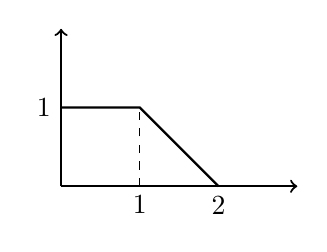
\begin{tikzpicture}
        \draw[thick,->] (0,0) -- (0,2);
        \draw[thick,->] (0,0) -- (3,0);
        \draw[thick] (0,1) node[anchor=east] {1} -- (1,1) -- (2,0) node[anchor=north] {2};
        \draw[dashed] (1,0) node[anchor=north] {1} -- (1,1);
    \end{tikzpicture}
\end{center}
\begin{align}
    f(t) &= \begin{cases} \Theta(t)-\Theta(t-1) \\ (2-t)\left[\Theta(t-1)-\Theta(t-2)\right] \\ 0\end{cases} \\
    f(t) &= \Theta(t) + (1-t)\Theta(t-1) + (t-2)\Theta(t-2) \\
    \La[f(t)] &= \La[1] - \La[(t-1)\Theta(t-1)] + \La[(t-2)\Theta(t-2)] \\
              &= \La[1] - e^{-s}\La[t] + e^{-2s}\La[t] \\
              &= \frac1s - \frac{e^{-s}}{s^2} + \frac{e^{-2s}}{s^2}
\end{align}

Another useful trick:
\begin{align}
    \La[tf(t)] &= \ofnt t\,f(t)e^{-ts}dt \\ 
               &= -\ofnt f(t)\frac{de^{-ts}}{ds}dt \\
               &= -\frac{d}{ds} \left(\ofnt f(t)e^{-ts}dt\right) \\
               &= -\frac{d}{ds} \big(\La[f(t)]\big) \\
    \La[t^nf(t)] &= (-1)^n \frac{d^n}{ds^n}\big(\La[f(t)]\big) \\
    \La[1] &= \frac1s \\
    \La[t] &= \frac{1}{s^2} = -1\frac{d}{ds}\big(\La[1]\big) = \frac{1}{s^2} 
\end{align}

\section{Periodic Functions}
Consider $f(t)$, periodic with period $p$.
\begin{align}
    \La[f(t)] &= \ofnt f(t)e^{-ts}dt \\
              &= \int_0^p f(t)e^{-ts}dt + \int_p^{2p} f(t)e^{-ts}dt + \cdots + \int_{np}^{(n+1)p}f(t)e^{-ts}dt + \cdots
\end{align}
Shift, $t=x+np$, $x=0\to t=np,~ x=p\to t=(n+1)p$.
\begin{align}
    \int_0^p f(x+np)e^{-(x+np)s}dx &= e^{-snp}\int_0^p f(x)e^{-xs}dx \\
    \La[f(t) &= \left(\int_0^p f(x)e^{-xs}dx\right)\left[1+e^{-ps}+\cdots+e^{-nps}+\cdots\right] \\
             &= \frac{1}{1-e^{-ps}} \int_0^p f(x)e^{-xs}dx
\end{align}

\begin{example}
Consider
\begin{align}
    f(t) &= \begin{cases}1 & n+0 < t < n+1 \\ 0 & n+1 < t < n+2 \end{cases}
\end{align}
Period, $p=2$.
\begin{align}
    \La[f(t)] &= \frac{1}{1-e^{-2s}} \int_0^2 f(t)e^{-st}dt \\
              &= \frac{1}{1-e^{-2s}} \int_0^1 e^{-st}dt \\
              &= \frac{1-e^{-s}}{s(1-e^{-2s})} 
\end{align}
\end{example}

\section{Laplace transform of delta function}
\begin{align}
    \La[\delta(t-t')] &= e^{-t's},~ t'>0,s> 0 \\
    \La[\delta(t)] &= 1 
\end{align}

Consider Newton's second law, applied to an instantaneous impulse:
\begin{align}
    m\ddot{x} &= \unl{p}\delta(t),~ x(0)=x_0,\dot{x}(0)=v_0 \\
    \La[m\ddot{x}] &= \La[p\delta(t)] \\
    m\big(s^2\La[x] - sx(0) - \dot{x}(0)\big) &= \unl{p} \\
    \La[x] &= \left(\frac{p}{m} + v_0\right)\frac{1}{s^2} + \frac{x_0}{s} \\
    x(t) &= \left(\frac{p}{m} + v_0\right)t + x_0
\end{align}

\section{Convolution Theorem}
\begin{align}
    (f\times g) &= \int_0^t f(x)g(t-x)\,dx \\
    \La[f\times g] &= \La[f]\La[g] \\
    \La[f\times g] &= \ofnt \left(\int_0^t f(x)g(t-x)\;dx\right) e^{-st}dt \\
                   &= \ofnt \left(\int_x^\infty f(x)g(t-x)\;e^{-ts}dt\right)\;dx,~ y=t-x,\,dy=dt \\
                   &= \ofnt \left(\ofnt f(x)g(y)e^{-(y+x)s}dy\right)\; dx \\
                   &= \left(\ofnt f(x)e^{-xs}dx\right)\cdot \left(\ofnt g(y)e^{-ys}dy\right) = \La[f]\cdot\La[g]
\end{align}

A useful tool for integrals:
\begin{align}
    I(x) &= \int_0^x \cos\big(b(x-u)\big)e^{au}\,du
\end{align}

\chapter{}
\section{Solving Differential Equations with Laplace Transforms}
\begin{align}
    \La\left[\frac{d^n}{dt^n}f(t)\right] &= s^n\La[f(t)] - \sum_{k=0}^{n-1} s^{n-1-k}f^{(k)}(0) \\
    \La[f(t-a)\Theta(t-a)] &= e^{-as}\La[f(t)]
\end{align}

\begin{example}
Consider:
\begin{align}
    y'' &+ 3y' + 2y = 2 - 2\Theta(t-1) \\
    y(0) &= 0,~ y'(0) = 2 \\
    \La[y''] &= s^2\bar{y} - sy(0) - y'(0) = s^2\bar{y} - 2 \\
    \La[y'] &= s\bar{y} - y(0) = s\bar{y} \\
    \La[2] &= \frac{2}{s} \\
    \La[\Theta(t-1)] &= \frac{e^{-s}}{s} \\
    s^2\bar{y} - 2 &+ 3s\bar{y} + 2\bar{y} = \frac{2}{s} - \frac{e^{-s}}{s} \\
    \bar{y}(s^2 &+ 3s + 2) = 2\left(1 + \frac{1}{s} - \frac{2e^{-s}}{s}\right) \\
    \bar{y}(s &+1)(s+2) = 2\left(1+\frac{1}{s}-\frac{2e^{-s}}{s}\right) \\
    \bar{y} &= \frac{2}{(s+1)(s+2)}\left(\frac{s+1}{s}-\frac{2e^{-s}}{s}\right) \\
            &= \frac{2}{s(s+2)} - \frac{2e^{-s}}{s(s+1)(s+2)} \\
            &= \frac{1}{s}-\frac{1}{s+1} - e^{-s}\left(\frac{1}{s} - \frac{2}{s+1} + \frac{1}{s+2}\right) \\
    y(t) &= 1 - e^{-2t} - \Theta(t-1) \left(1-2e^{-(t-1)} + e^{2(t-1)}\right)
\end{align}
\end{example}

\section{Coupled Differential Equations}
\begin{example}[Electrical circuits]
\begin{align}
    L\ddot{q}_1 &+ M\ddot{q}_2 + \frac{1}{c}q_1 = 0 \\
    M\ddot{q}_1 &+ L\ddot{q}_2 + \frac{1}{c}q_2 = 0 \\
    q_1(0) &= \dot{q}_1(0) = \ddot{q}_2(0) = 0 \\
    q_2(0) &= V_0C \\
    \La[\ddot{q}_1] &= s^2\La[q_1] - \dot{q}_1(0) - sq_1(0) = s^2\La[q_1] \\
    \La[\ddot{q}_2] &= s^2\La[q_2] V_0Cs \\
    \La[q_1]\left(Ls^2+\frac{1}{c}\right) &+ \La[q_2]s^2M = sMV_0C \\
    \La[q_1]s^2M &+ \La[q_2]\left(Ls^2+\frac{1}{c}\right) = sLV_0C \\
    \La[q_1] &= \frac{V_0C}{2} \left[\frac{(L+M)s}{(L+M)s^2 + \frac{1}{c^2}} - \frac{(L-M)s}{(L-M)s^2+\frac{1}{c^2}}\right], \approx \frac{s}{s^2+a^2} \\
    q_1(t) &= \frac{V_0C}{2}\left[\cos\left(\frac{t}{\sqrt{(L+M)c^2}}\right) - \cos\left(\frac{t}{\sqrt{(L-M)c^2}}\right)\right]
\end{align}
\end{example}

\textbf{Theorem:} Suppose that $\La[f](s)$ admits a series expansion of the form:
\begin{align}
    \La[f](s) &= \sum_{n=0}^\infty a_n s^{-n-1},\; |s|>f 
\end{align}
Then, for $t>0$:
\begin{align}
    f(t) &= \sum_{n=0}^\infty \frac{a_n}{n!} t^n
\end{align}

\begin{example}
\begin{align}
    ty'' &+ y' + ty - 0 \\
    y(0) &= 1,\; y'(0) = 0 \\
    \La[ty] &= -\frac{d}{ds}\bar{y} \\
    \La[y'] &= s\bar{y} - y(0) = s\bar{y} - 1 \\
    \La[ty''] &= -\frac{d}{ds}\left(\La[y'']\right) = -\frac{d}{ds}\left(s^2\bar{y} - sy(0) - y'(0)\right) \\
              &= -\left(2s\bar{y}+s^2\frac{d}{ds}\bar{y}-1\right) \\
    -\left(2s\bar{y}+s^2\frac{d}{ds}\bar{y}-1\right) &+ s\bar{y} - 1 - \frac{d}{ds}\bar{y} = 0 \\
    -\frac{d}{ds}\bar{y}(s^2+1) &- s\bar{y} = 0 \\
    \frac{d}{ds}\bar{y} &= \frac{-s}{s^2+1}\bar{y} \\
    \int \frac{d\bar{y}}{\bar{y}} &= \int \frac{-s\,ds}{s^2+1} \\
    \log\bar{y} &= C - \frac12\log\left(s^2+1\right) \\
    \bar{y} &= \frac{C}{\sqrt{s^2+1}},~ |s|>1 \\
    \bar{y} &= \frac{C}{s\sqrt{1+\frac{1}{s^2}}} = \sum_{n=0}^\infty \frac{(-1)^n (2n)!}{(n!)^2 2^{2n}} \frac{1}{s^{2n+1}} \\
    y(t) &= \sum_{n=0}^\infty \frac{(-1)^n}{(n!)^2} \frac{t^{2n}}{2^{2n}} = J_0(t)
\end{align}
\end{example}

\chapter{}
\section{Inverting the Laplace Transform}
Inspirations:
\begin{itemize}
    \item Inspection
    \item Convolution Theorem
\end{itemize}
Perspiration:
\begin{itemize}
    \item Inverse Laplace Transform - Bromwich integral
\end{itemize}

\subsection{Inspection}
\begin{align}
    \La[1] &= \frac1s \\
    \La[t^n] &= \frac{n!}{s^{n+1}} \\
    \La[e^{at}] &= \frac{1}{s-a}
\end{align}

\begin{example}
\begin{align}
    \La[f](s) &= \frac{4}{s(s+2)} = \frac2s - \frac{2}{s+2} \\
              &= 2\La[1] - 2\La[e^{-2t}] \\
    f(t) &= 2-2e^{-2t}
\end{align}
\end{example}

\subsection{Convolution}
\begin{align}
    (f\times g) &= \int_0^t f(x)g(t-x)\,dx \\
    \La[f\times g] &= \La[f]\cdot\La[g]
\end{align}

\begin{example}
\begin{align}
    \La[f](s) &= \frac{4}{s^2(s+2)^2} \\
    \frac{1}{s^2} &= \La[t](s) \\
    \frac{1}{(s+2)^2} &= -\frac{d}{ds}\left(\frac{1}{s+2}\right) = -\frac{d}{ds}\left(\La[e^{-2t}]\right) \\
                      &= \La[te^{-2t}](s) \\
    \La[f](s) &= 4\La[t]\cdot\La[te^{-2t}] = 4\La[t\times te^{-2t}] \\
    f(t) &= 4\left(t\times te^{-2t}\right) \\
         &= 4\int_0^t x(t-x)e^{-2(t-x)}dx = (1+t)e^{-2t} + t - 1
\end{align}
This could have been done in other ways:
\begin{align}
    \La[f](s) &= \frac{4}{s^2(s+2)^2} \\
              &= \frac14 \frac{4}{s(s+2)} \cdot \frac{4}{s(s+2)} \\
              &= \frac14 \La[2-2e^{-2t}]\cdot\La[2-2e^{-2t}] \\
              &= \frac14 \La[(2-2e^{-2t}\times(2-2e^{-2t})] \\
    f(t) &= \frac14 \left((2-2e^{-2t})\times(2-2e^{-2t})\right)
\end{align}
\end{example}

\subsection{Inversion Theorem}
Consider a function $f(t)$ which is piece smooth in $[0,\infty]$ and whose Laplace transform $\La[f(t)](s)$ exists for $\text{Re}(s)>0$, then
\begin{align}
    f(t) &= \frac{1}{2\pi i} \int_{\sigma-i\infty}^{\sigma+i\infty} \La[f](s)e^{st}ds.
\end{align}
\textbf{Proof:}\\
First consider $s=\sigma+ix$.
Now recall
\begin{align}
    \La[f](s) &= \sqrt{2\pi}\F^{-1}[f(t)\Theta(t)e^{-\sigma t}](x) \\
    f(t)\Theta(t)e^{-\sigma t} &= \frac{1}{\sqrt{2\pi}} \F[\La[f](s)](t) \\
                               &= \frac{1}{2\pi} \ifnt \La[f](\sigma + ix)e^{ixt}dx \\
    f(t)\Theta(t) &= \frac{1}{2\pi} \ifnt \La[f](\sigma+ix)e^{(\sigma+ix)t}dx \\
                  &= \frac{1}{2\pi i} \int_{\sigma-i\infty}^{\sigma+i\infty} \La[f](s)\,e^{st}ds
\end{align}
If $\La[f]$ is a meromorphic function with a finite number of poles $\{a_i\},i=\{1\dots,n\}$.
The key thing is that the singularities are finite, therefore $\exists M \in \R \; / \; |\La[f](s)| \leq M|s|^{-k}$.
We choose $t>0,\sigma>\text{Re}(a_i)$, and due to the positive exponential, we choose the left handside of the line from $\sigma-i\infty \to \sigma+i\infty$ to close the contour.
\begin{align}
    f(t) &= \frac{1}{2\pi i} \int_{\sigma-i\infty}^{\sigma+i\infty} \La[f](s)\,e^{st}ds \\
         &= \sum_{i=1}^n \text{Res}\left[\La[f](s)\,e^{st}\right]\bigg|_{a_i}
\end{align}
The integral along the curve, $C_R$, vanishes:
\begin{align}
    \lim_{R\to\infty} \Bigg|\int_{C_R}\Bigg| &= 0
\end{align}
Parameterisation, $C_R:~ \sigma + Re^{i\theta},\; \theta \in \left[\frac{\pi}{2},\frac{3\pi}{2}\right]$
\begin{align}
    |s| = |\sigma + Re^{i\theta}| &\geq \big| |\sigma| - |Re^{i\theta}|\big| \\
                                  &= |\sigma - R| = R-\sigma
\end{align}
Now show, using the same definition of $s$:
\begin{align}
    \Bigg| \frac{1}{2\pi i} \int_{C_R} \La[f](s)\,e^{st}ds\Bigg| &= \Bigg| \frac{1}{2\pi i} \int_{\pi/2}^{3\pi/2} \La[f](\sigma+Re^{i\theta})\, e^{(\sigma+Re^{i\theta})t} iRe^{i\theta}\,d\theta \Bigg|\\
                                                                 &\leq \frac{1}{2\pi} \int_{\pi/2}^{3\pi/2} \bigg|\La[f](\sigma+Re^{i\theta})\bigg|\;\bigg|e^{(\sigma+Re^{i\theta})t}iRe^{i\theta}\bigg|\,d\theta \\
    \bigg| \La[f](\sigma+Re^{i\theta})\bigg| &\leq M|s|^{-k} \\
                                             &\leq M(R-\sigma)^{-k} \\
    \bigg| e^{t(\sigma+Re^{i\theta})}\bigg| &= \bigg|e^{t(\sigma+R\cos\theta)}e^{itR\sin\theta}\bigg| \\
                                            &= e^{t(\sigma+R\cos\theta)} \\
    \Bigg| \frac{1}{2\pi i} \int_{C_R} \La[f](s)\,e^{st}ds\Bigg| &< \frac{1}{2\pi} \int_{\pi/2}^{3\pi/2} M(R-\sigma)^{-k}\,e^{t(\sigma+R\cos\theta)}R\,d\theta \\
    \lim_{R\to\infty} &\to 0
\end{align}
If instead you want to calculate for $-t$, you choose $\sigma < \text{Re}(a_i)$ and integrate over a contour to the right.

\begin{example}
\begin{align}
    \La[f](s) &= \frac{4}{s^2(s+2)^2}
\end{align}
We have double poles at $0$ and $-2$.
Use above method, integrate to the right of these, and close the circle on the left enclosing the pooles.
\begin{align}
    f(t)_{t>0} &= \text{Res}\left[\frac{4}{s^2(s+2)^2}e^{st}\right]_{s=0} + \text{Res}\left[\frac{4}{s^2(s+2)^2}e^{st}\right]_{s=-2} 
\end{align}
For a pole of order m,
\begin{align}
    \text{Res}[f(z)]_{z=z_0} &= \frac{1}{(m-1)!} \frac{d^{m-1}}{dz^{m-1}} \left[(z-z_0)^mf(z)\right]_{z=z_0}
\end{align}
So, (8.41) simplifies to
\begin{align}
    f(t) &= t-1+e^{-2t}(1+t)
\end{align}
\end{example}

\chapter{Fourier Transforms and Quantum Mechanics}

\textbf{Note: Calculating residues for second and third order poles will be on the exam.}\\
$f(x)$ is square-integrable:
\begin{equation}
    \ifnt |f(x)|^2\,dx < \infty 
\end{equation}
The set of all square-integrable functions is denoted by the $\mathbb{L}^2$ Hilbert space with with the inner product,
\begin{equation}
    \langle f|g\rangle = \ifnt f(x)^*g(x)\,dx, 
\end{equation}
and the norm,
\begin{equation}
    ||f||^2 = \langle f|f\rangle = \ifnt |f(x)|^2\,dx < \infty
\end{equation}

Consider a linear operator, $\hat{F}[f(x)]$.
\begin{align}
    \hat{F}[f(x)](k) &= \frac{1}{\sqrt{2\pi}} \ifnt f(x) e^{-ikx}dx \\
                     &= \F^{-1}[f(x)](k) \\
    \hat{F}^{-1}[\bar{f}(k)](x) &= \F[\bar{f}(k)](x) \\
    \hat{F}f &= \bar{f} 
\end{align}
Here, $x$ is position space, and $k$ is momentum space.

\section{Parseval Function}
\begin{equation}
    \langle f|g\rangle = \langle \hat{F}f|\hat{F}g\rangle
\end{equation}
The Fourier transform preserves the scalar transform in $\mathbb{L}^2$.
$\hat{F}$ is a unitary operator, $\hat{F}^{-1} = \hat{F}^\dagger$.
The norm of a function is invariant under the transform.

\section{The Position and Momentum Operators}
Wave function,
\begin{align}
    \psi(x) &\in \R^2 \\
    ||\psi(x)|| &= 1 
\end{align}
$|\psi(x)|^2$ is the probability density of finding a particle in position $x$.

What is the meaning of $\hat{F}\psi = \bar{\psi}$?\\
The momentum operator, 
\begin{equation}
    \hat{p} = -i\frac{\p}{\p x},
\end{equation}
has eigenvalues $\phi \in \R$, and eigenvectors,
\begin{align}
    \Phi_p(x) &= \frac{1}{\sqrt{2\pi}} e^{\phi x}.\\
    \hat{p}\Phi_p(x) &= p_0\Phi_p(x) \\
    |\langle\phi_p|\psi\rangle|^2 &= \Bigg|\ifnt \frac{dx}{\sqrt{2\pi}} \psi(x)e^{-ip_0x}\Bigg|^2\\
                                  &= |\hat{F}\psi(x)|^2 \\
                                  &= |\bar{\psi}(p_0)|^2
\end{align}
This is the wavefunction in momentum space.
\begin{align}
    ||\psi|| &= ||\bar{\psi}|| = 1 \\
    \hat{p}\bar{\psi}(p) &= \hat{F}[\hat{p}\psi(p^*)] \\
                         &= \hat{F}[-i\frac{\p}{\p x} \psi(x)] \\
                         &= -iip\bar{\psi}(p) \\
                         &= \unl{p}\bar{\psi}(p) \\
    \bar{\Phi}_p(p) &= \hat{F}[\Phi_p(x)] \\
                    &= \hat{F}\left[\frac{1}{\sqrt{2\pi}} e^{ipx}\right] \\
                    &= \frac{1}{\sqrt{2\pi}} \ifnt \frac{1}{\sqrt{2\pi}} e^{-i(p-p_0)x}dx \\
                    &= \delta(p-p_0)\\
    \hat{p}\Phi_p(p) &= p\bar{\Phi}_p(p) \\
                       &= p\delta(p-p_0)\\
                       &= p_0\bar{\Phi}_p(p)
\end{align}

\section{Position operator}
Defined in position space as
\begin{equation}
    \hat{x}\psi(x) = x\psi(x).
\end{equation}
Its eigenfunctions are delta functions, $\chi_{x_0} = \delta(x-x_0)$.
So in momentum space, 
\begin{align}
    \hat{x}\bar{\psi}(p) &= \hat{F}[\hat{x}\psi(x)] = i\frac{\p}{\p p}\bar{\psi}(p) \\
    \bar{\chi}_{x_0} &= \hat{F}(\delta(x-x_0)) \\
                     &= \frac{1}{\sqrt{2\pi}} \ifnt \delta(x-x_0)e^{-ipx} dx = \frac{1}{\sqrt{2\pi}} e^{-ipx_0}
\end{align}
\begin{center}
    \begin{tabular}{c|c}
        Configuration Space & Momentum Space \\
        \hline
        $\psi(x)$ & $\bar{\psi}(x) = \hat{F}[\psi(x)](p)$ \\
        $\hat{x} = x$ & $i\frac{\p}{\p p}$ \\
        $\hat{p} = -i\frac{\p}{\p x}$ & $p$ \\
        $\Phi_{p_0}(x) = \frac{1}{\sqrt{2\pi}}e^{ip_0 x}$ & $\bar{\Phi}_{p_0}(p) = \delta(p-p_0)$ \\
        $\chi_{x_0} = \delta(x-x_0)$ & $\bar{\chi}_{x_0}(p) = \frac{1}{\sqrt{2\pi}}e^{-ipx_0}$
    \end{tabular}
\end{center}

\chapter*{Table of Laplace Transforms}
\begin{center}
    \begin{tabular}{c|c}
        $f(t)$ & $\bar{f}(s)$ \\
        \hline
        1 & $\frac{1}{s}$  \\
        $t$ & $\frac{1}{s^2}$  \\
        $t^n$ & $\frac{n!}{s^{n+1}}$  \\
        $e^{at}$ & $\frac{1}{s-a}$  \\
        $\sin(wt)$ & $\frac{w}{s^2+w^2}$  \\
        $\cos(wt)$ & $\frac{s}{s^2+w^2}$  \\
        $t^ng(t)$ & $(-1)^n\frac{d^nG(s)}{ds^n}$  \\
        $t\sin(wt)$ & $\frac{2ws}{(s^2+w^2)^2}$  \\
        $t\cos(wt)$ & $\frac{s^2-w^2}{(s^2+w^2)^2}$  \\
        $g(at)$ & $\frac{1}{a}G\left(\frac{s}{a}\right)$  \\
        $e^{at}g(t)$ & $G(s-a)$  \\
        $t^ne^{at}$ & $\frac{n!}{(s-a)^{n+1}}$  \\
        $te^{-t}$ & $\frac{1}{(s+1)^2}$  \\
        $1-e^{-t/T}$ & $\frac{1}{s(1+Ts)}$ \\
        $e^{at}\sin(wt)$ & $\frac{w}{(s-a)^2+w^2}$  \\
        $e^{at}\cos(wt)$ & $\frac{s-a}{(s-a)^2+w^2}$  \\
        $g'(t)$ & $sG(s) - g(0)$  \\
        $g''(t)$ & $s^2G(s) - sg(0) - g'(0)$  \\
        $g^{(n)}(t)$ & $s^nG(s) - \sum_{k=0}^{n-1} s^{n-1-k}g^{(k)}(0)$ \\
        $\int_0^t g(t)\,dt$ & $\frac{G(s)}{s}$  \\
        $\int g(t)\,dt$ & $\frac{G(s)}{s} + \frac1s\left\{\int g(t)\,dt\right\}_{t=0}$  
    \end{tabular}
\end{center}
\end{document}
